\documentclass[dvipsnames]{standalone}
\usepackage{tikz}

\usetikzlibrary{positioning}
\usetikzlibrary{calc}

\colorlet{line2line}{SkyBlue!50}

\newcommand{\stheight}{0.7cm}
\newcommand{\stshift}{0.3cm}
\newcommand{\labeloffset}{2cm}

\begin{document}

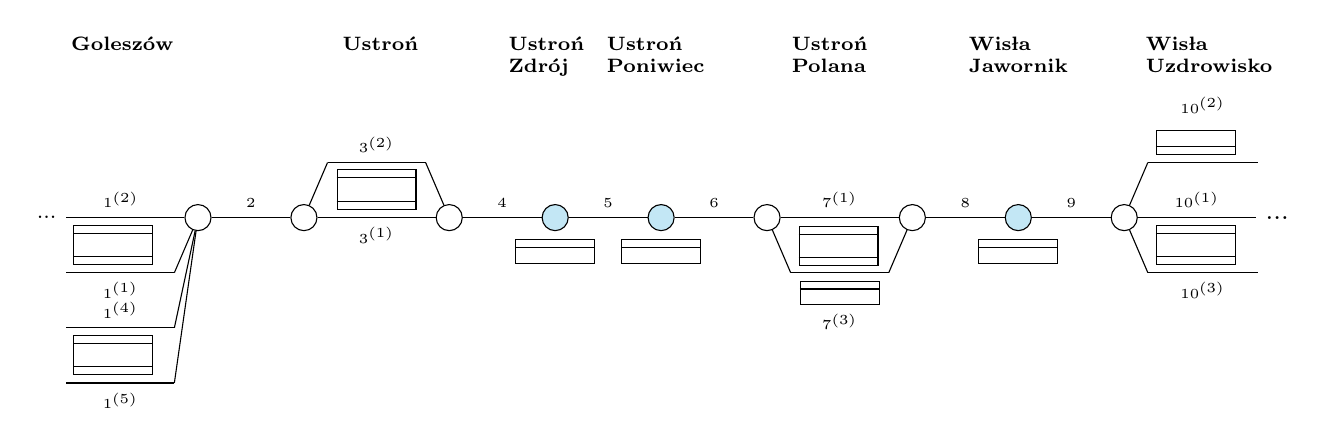
\begin{tikzpicture}[
  junction/.style={draw,circle},
  station/.style={text=black, font={\bfseries \scriptsize}},
    onesideplatform/.pic={
        \node[
            draw,rectangle,minimum height=0.3cm, minimum width=1cm
        ] (platform) {};
        \coordinate [above=0.05cm of platform.west] (x);
        \coordinate [above=0.05cm of platform.east] (y);
        \draw (x) -- (y);
    },
    bottomonesideplatform/.pic={
        \node[
            draw,rectangle,minimum height=0.3cm, minimum width=1cm
        ] (platform) {};
        \coordinate [below=0.05cm of platform.west] (x);
        \coordinate [below=0.05cm of platform.east] (y);
        \draw (x) -- (y);
    },
    twosideplatform/.pic={
        \node[
            draw,rectangle,minimum height=0.5cm, minimum width=1cm
        ] (platform) {};
        \coordinate [above=0.15cm of platform.west] (x);
        \coordinate [above=0.15cm of platform.east] (y);
        \coordinate [below=0.15cm of platform.west] (u);
        \coordinate [below=0.15cm of platform.east] (v);
        \draw (x) -- (y);
        \draw (u) -- (v);
    }
]

\node [] (start) {\footnotesize ...};
\node [junction, right=1.5cm of start] (A) {};
\node [junction, right=1cm of A] (AA) {};
\node [junction, right=1.5cm of AA] (AAA) {};
\node [junction, right=1cm of AAA, fill=line2line] (B) {};
\node [junction, right=1cm of B, fill=line2line] (C) {};
\node [junction, right=1cm of C] (D) {};
\node [junction, right=1.5cm of D] (E) {};
\node [junction, right=1cm of E, fill=line2line] (F) {};
\node [junction, right=1cm of F] (G) {};
\node [right=1.5cm of G] (stop) {...};
\node [station,above=\labeloffset of $(start)!0.5!(A)$] (goleszow) {Goleszów};
\node [station,base right=1.9cm of goleszow] (ustron) {Ustroń};
\node [text width=1.3cm, station,base right=0.9cm of ustron] (uz) {Ustroń\\Zdrój};
\node [text width=1.3cm, station,base right=-0.3cm of uz] (up) {Ustroń\\Poniwiec};
\node [text width=2cm, station,base right=0.8cm of up] (upo) {Ustroń\\Polana};
\node [text width=2cm, station,base right=0.0cm of upo] (wj) {Wisła\\Jawornik};
\node [text width=2cm, station,base right=0.0cm of wj] (wj) {Wisła\\Uzdrowisko};

\draw (start) -- (A) node[midway,above left=0.0cm and -0.29cm]{\tiny $1^{(2)}$};
\draw (A) -- (AA) node[midway,above]{\tiny $2$};
\draw (AA) -- (AAA) node[midway,below]{\tiny $3^{(1)}$};
\draw (AAA) -- (B) node[midway,above]{\tiny $4$};
\draw (B) -- (C) node[midway,above]{\tiny $5$};
\draw (C) -- (D) node[midway,above]{\tiny $6$};
\draw (D) -- (E) node[midway,above]{\tiny $7^{(1)}$};
\draw (E) -- (F) node[midway,above]{\tiny $8$};
\draw (F) -- (G) node[midway,above]{\tiny $9$};
\draw (G) -- (stop) node[midway,above]{\tiny $10^{(1)}$};


\coordinate [below right=3*\stheight and 0.25cm of start.center] (start1);
\coordinate [below left=3*\stheight and \stshift of A.center] (A1);
\draw (start1) -- (A1) node[midway, below]{\tiny $1^{(5)}$};
\draw (A1) -- (A);

\coordinate [below right=\stheight and 0.25cm of start.center] (start2);
\coordinate [below left=\stheight and \stshift of A.center] (A2);
\draw (start2) -- (A2) node[midway, below]{\tiny $1^{(1)}$};
\draw (A2) -- (A);

\coordinate [below right=2*\stheight and 0.25cm of start.center] (start3);
\coordinate [below left=2*\stheight and \stshift of A.center] (A3);
\draw (start3) -- (A3) node[midway, above]{\tiny $1^{(4)}$};
\draw (A3) -- (A);

\coordinate [below right=\stheight and \stshift of D.center] (D1);
\coordinate [below left=\stheight and \stshift of E.center] (E1);
\draw (D) -- (D1);
\draw (D1) -- (E1) node[midway,below=0.4cm]{\tiny $7^{(3)}$};
\draw (E1) -- (E);

\coordinate [above right=\stheight and \stshift of AA.center] (AA1);
\coordinate [above left=\stheight and \stshift of AAA.center] (AAA1);
\draw (AA) -- (AA1);
\draw (AA1) -- (AAA1) node[midway,above]{\tiny $3^{(2)}$};
\draw (AAA1) -- (AAA);

\coordinate [below left=\stheight and 0.25cm of stop.center] (stop1);
\coordinate [below right=\stheight and \stshift of G.center] (G1);
\draw (G) -- (G1);
\draw (G1) -- (stop1) node[midway,below]{\tiny $10^{(3)}$};


\coordinate [above left=\stheight and 0.25cm of stop.center] (stop2);
\coordinate [above right=\stheight and \stshift of G.center] (G2);
\draw (G) -- (G2);
\draw (G2) -- (stop2) node[midway,above=0.5cm]{\tiny $10^{(2)}$};

\pic [below=0.1cm of B] {onesideplatform};
\pic [below=0.1cm of C] {onesideplatform};

\pic [below left=1.365cm and 0.45cm of A] {twosideplatform};
\pic [below left=-0.03cm and 0.45cm of A] {twosideplatform};

\pic [below right=-0.02cm and 0.28cm of D] {twosideplatform};

\pic [above=0.1cm of $(AA)!0.5!(AAA)$] {twosideplatform};

\pic [below=0.1cm of C] {onesideplatform};
\pic [below=0.8cm of $(D)!0.5!(E)$] {onesideplatform};

\pic [below right=-0.03cm and 0.28cm of G] {twosideplatform};
\pic [above right=0.675cm and 0.28cm of G] {bottomonesideplatform};

\pic [below=0.1cm of F] {onesideplatform};
\end{tikzpicture}


\end{document}
